% ---------------------------------------------------------------------------- %
\chapter{Resultados}
\label{cap:resultados}
% ---------------------------------------------------------------------------- %

Em dezembro de 2016 o protótipo de \textit{PsyChO: The Ball} foi finalizado, e teve seu primeiro lançamento no evento expositivo da \textit{UspGameDev}. Nele vários alunos da \textit{USP} puderam comparecer e jogá-lo gratuitamente, dentre outros jogos de membros do grupo de extensão. Foi uma imensa satisfação observar outras pessoas jogando e se divertindo com o jogo, mesmo ele sendo um protótipo.

Uma das maiores importâncias nesses eventos é poder receber \textit{feedback} de outras pessoas como opiniões sobre caracterícticas, descobrir se os conceitos de design escolhidos funcionaram ou não, e até mesmo descobrir novos \textit{bugs}. Isso facilita imensamente o segundo passo após uma exposição de polir e consertar onde for necessário.

% ---------------------------------------------------------------------------- %
\section{Conteúdo}
\label{sec:conteudo}

\begin{figure}[h!]
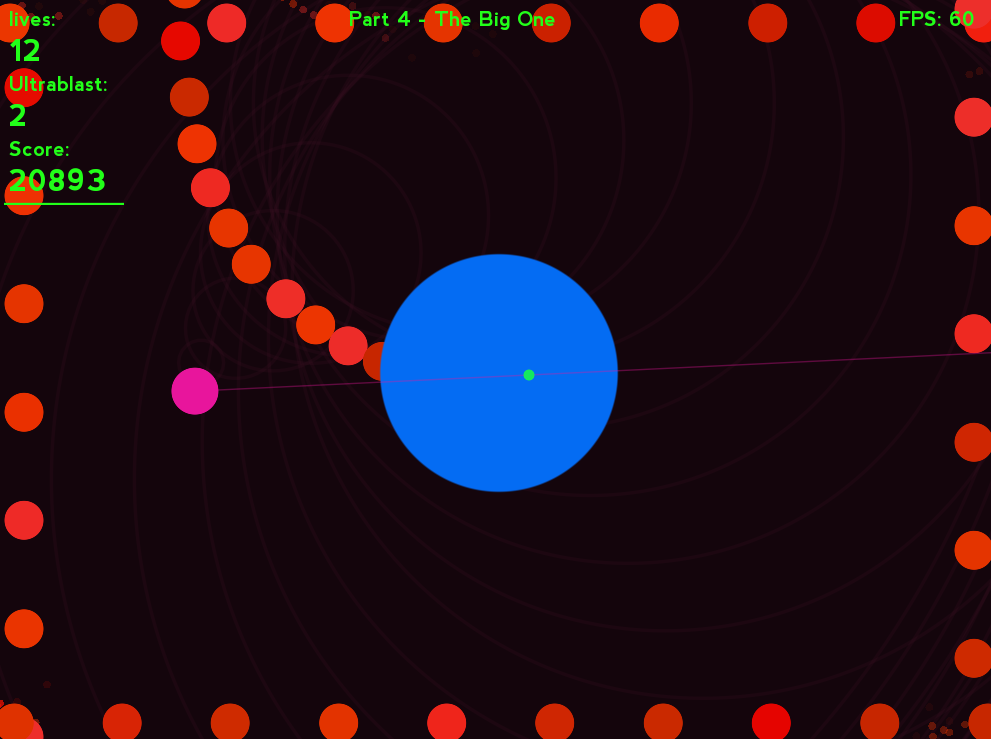
\includegraphics[scale=.35]{ss1}
\centering
\caption{Primeiro chefão do jogo atacando o jogador}
\end{figure}

O jogo em seu estado atual possui 2 níveis dos 5 planejadas. Cada nível tem sua própria trilha sonora, e é divido em quatro partes únicas, sendo a última composta por um \textit{chefão}. O jogo é composto de vários efeitos especiais visuais e sonoros, e abrange 5 inimigos diferentes para desafiar o jogador.\\

\begin{figure}[h!]
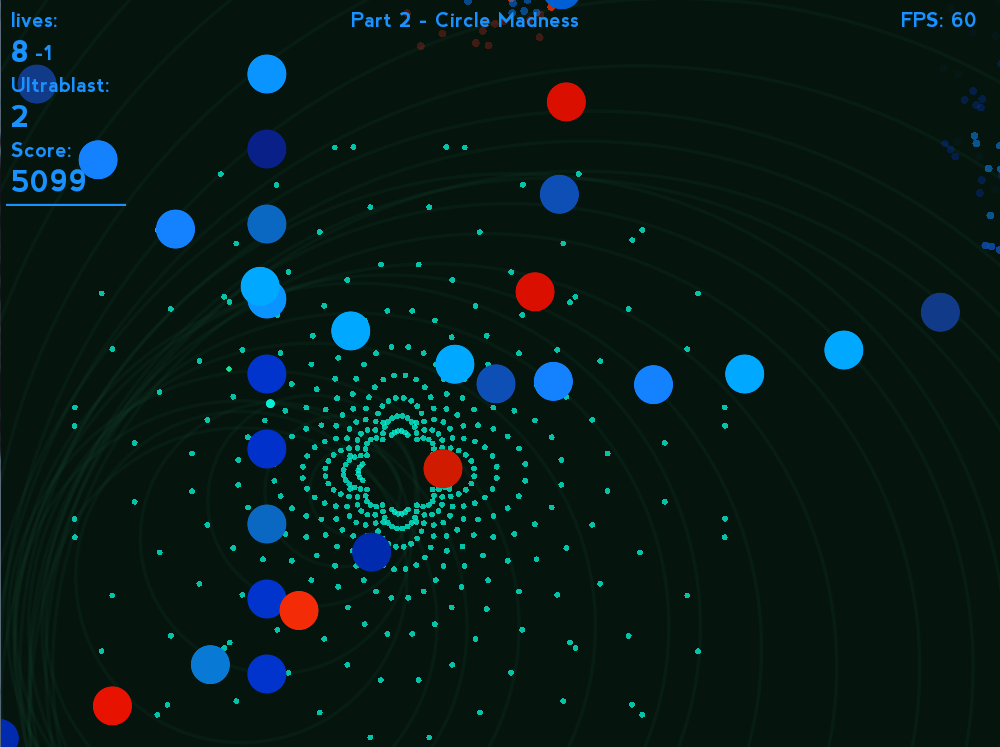
\includegraphics[scale=.35]{ss4}
\centering
\caption{Jogador morrendo para uma onda de inimigos lhe atacando}
\end{figure}

Além disso o jogo salva as maiores pontuações entre partidas, então jogadores podem sempre tentar superar a pontuação de colegas, ou tentar aumentar seu próprio recorde.
O sistema para rodar níveis através de scripts permite facilmente que usuários criem e joguem seus pŕoprios níveis sem precisar de muito conhecimento computacional.

% ---------------------------------------------------------------------------- %
\section{Eventos}
\label{sec:eventos}

%Falar dos eventos que levei (lets play 1 (dezembro de 2016), lets play 2 (2017) com melhorias depois de feedback). Mostrar umas fotos de pessoas jogando, e como eu quis colocar a %mecanica de highscore graças ao feedback. Falar como nesses eventos achavam bugs que pude consertar depois (ou na hora)

% ---------------------------------------------------------------------------- %
\section{Como Jogar}
\label{sec:how_to_play}

%Colocar links onde da pra baixar e jogar o jogo.

Para jogador o jogo, está disponivel online uma página com todos os lançamentos do jogo em seu próprio repositório no domínio \textit{Github}:
\\~\\
\url{https://github.com/uspgamedev/Project-Telos/releases}
\\~\\
Neste link você encontra instruções de como instalar e jogar \textit{PsyChO: The Ball} nos sistemas operacionais \textit{Linux} (suporte direto para distros baseadas em \textit{Ubuntu} ou \textit{Debian}), \textit{Windows} ou \textit{Macintosh}.
\\~\\
Além disso você pode acessar diretamente o código fonte e rodar você mesmo através da página principal do repositório do projeto:
\\~\\
\url{https://github.com/uspgamedev/Project-Telos/}
